\documentclass[1p]{elsarticle_modified}
%\bibliographystyle{elsarticle-num}

%\usepackage[colorlinks]{hyperref}
%\usepackage{abbrmath_seonhwa} %\Abb, \Ascr, \Acal ,\Abf, \Afrak
\usepackage{amsfonts}
\usepackage{amssymb}
\usepackage{amsmath}
\usepackage{amsthm}
\usepackage{scalefnt}
\usepackage{amsbsy}
\usepackage{kotex}
\usepackage{caption}
\usepackage{subfig}
\usepackage{color}
\usepackage{graphicx}
\usepackage{xcolor} %% white, black, red, green, blue, cyan, magenta, yellow
\usepackage{float}
\usepackage{setspace}
\usepackage{hyperref}

\usepackage{tikz}
\usetikzlibrary{arrows}

\usepackage{multirow}
\usepackage{array} % fixed length table
\usepackage{hhline}

%%%%%%%%%%%%%%%%%%%%%
\makeatletter
\renewcommand*\env@matrix[1][\arraystretch]{%
	\edef\arraystretch{#1}%
	\hskip -\arraycolsep
	\let\@ifnextchar\new@ifnextchar
	\array{*\c@MaxMatrixCols c}}
\makeatother %https://tex.stackexchange.com/questions/14071/how-can-i-increase-the-line-spacing-in-a-matrix
%%%%%%%%%%%%%%%

\usepackage[normalem]{ulem}

\newcommand{\msout}[1]{\ifmmode\text{\sout{\ensuremath{#1}}}\else\sout{#1}\fi}
%SOURCE: \msout is \stkout macro in https://tex.stackexchange.com/questions/20609/strikeout-in-math-mode

\newcommand{\cancel}[1]{
	\ifmmode
	{\color{red}\msout{#1}}
	\else
	{\color{red}\sout{#1}}
	\fi
}

\newcommand{\add}[1]{
	{\color{blue}\uwave{#1}}
}

\newcommand{\replace}[2]{
	\ifmmode
	{\color{red}\msout{#1}}{\color{blue}\uwave{#2}}
	\else
	{\color{red}\sout{#1}}{\color{blue}\uwave{#2}}
	\fi
}

\newcommand{\Sol}{\mathcal{S}} %segment
\newcommand{\D}{D} %diagram
\newcommand{\A}{\mathcal{A}} %arc


%%%%%%%%%%%%%%%%%%%%%%%%%%%%%5 test

\def\sl{\operatorname{\textup{SL}}(2,\Cbb)}
\def\psl{\operatorname{\textup{PSL}}(2,\Cbb)}
\def\quan{\mkern 1mu \triangleright \mkern 1mu}

\theoremstyle{definition}
\newtheorem{thm}{Theorem}[section]
\newtheorem{prop}[thm]{Proposition}
\newtheorem{lem}[thm]{Lemma}
\newtheorem{ques}[thm]{Question}
\newtheorem{cor}[thm]{Corollary}
\newtheorem{defn}[thm]{Definition}
\newtheorem{exam}[thm]{Example}
\newtheorem{rmk}[thm]{Remark}
\newtheorem{alg}[thm]{Algorithm}

\newcommand{\I}{\sqrt{-1}}
\begin{document}

%\begin{frontmatter}
%
%\title{Boundary parabolic representations of knots up to 8 crossings}
%
%%% Group authors per affiliation:
%\author{Yunhi Cho} 
%\address{Department of Mathematics, University of Seoul, Seoul, Korea}
%\ead{yhcho@uos.ac.kr}
%
%
%\author{Seonhwa Kim} %\fnref{s_kim}}
%\address{Center for Geometry and Physics, Institute for Basic Science, Pohang, 37673, Korea}
%\ead{ryeona17@ibs.re.kr}
%
%\author{Hyuk Kim}
%\address{Department of Mathematical Sciences, Seoul National University, Seoul 08826, Korea}
%\ead{hyukkim@snu.ac.kr}
%
%\author{Seokbeom Yoon}
%\address{Department of Mathematical Sciences, Seoul National University, Seoul, 08826,  Korea}
%\ead{sbyoon15@snu.ac.kr}
%
%\begin{abstract}
%We find all boundary parabolic representation of knots up to 8 crossings.
%
%\end{abstract}
%\begin{keyword}
%    \MSC[2010] 57M25 
%\end{keyword}
%
%\end{frontmatter}

%\linenumbers
%\tableofcontents
%
\newcommand\colored[1]{\textcolor{white}{\rule[-0.35ex]{0.8em}{1.4ex}}\kern-0.8em\color{red} #1}%
%\newcommand\colored[1]{\textcolor{white}{ #1}\kern-2.17ex	\textcolor{white}{ #1}\kern-1.81ex	\textcolor{white}{ #1}\kern-2.15ex\color{red}#1	}

{\Large $\underline{12a_{0819}~(K12a_{0819})}$}

\setlength{\tabcolsep}{10pt}
\renewcommand{\arraystretch}{1.6}
\vspace{1cm}\begin{tabular}{m{100pt}>{\centering\arraybackslash}m{274pt}}
\multirow{5}{120pt}{
	\centering
	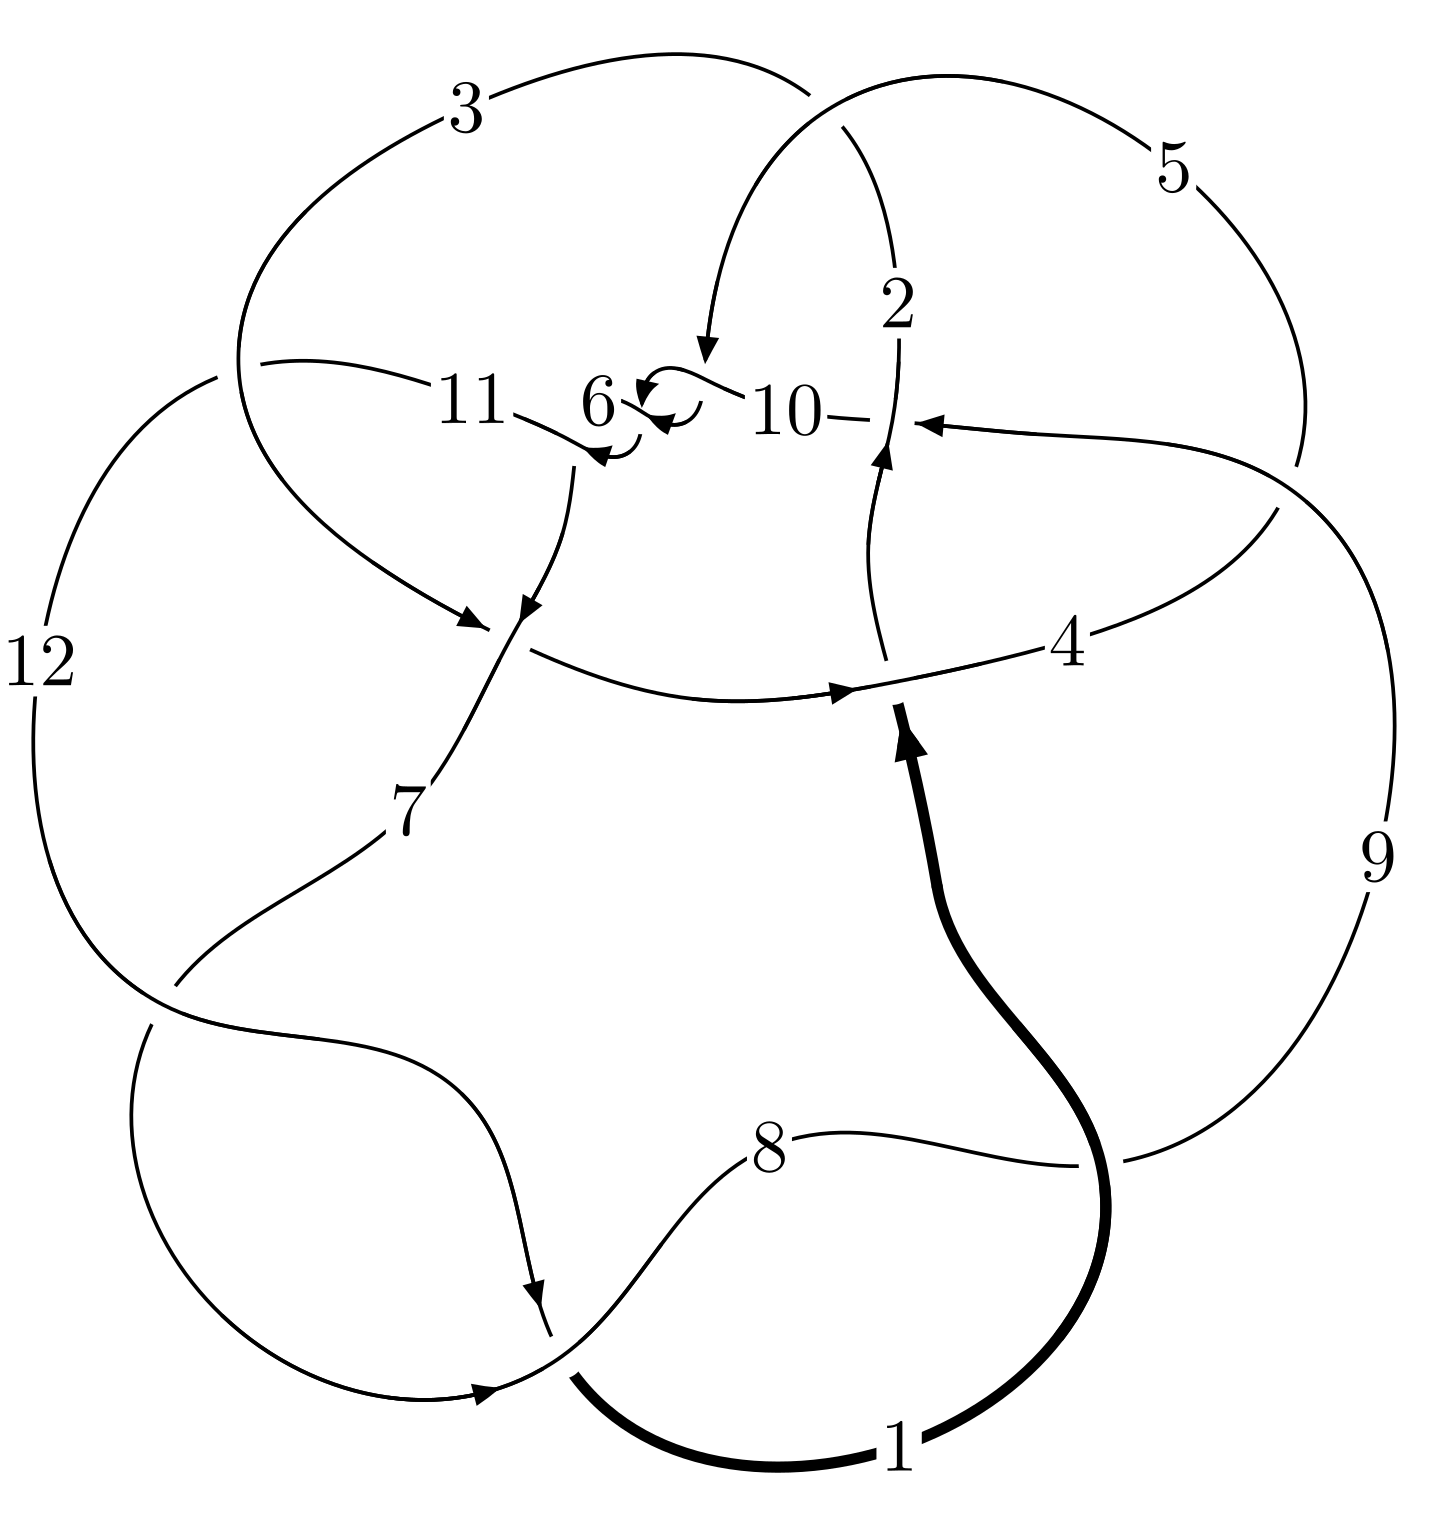
\includegraphics[width=112pt]{../../../GIT/diagram.site/Diagrams/png/1620_12a_0819.png}\\
\ \ \ A knot diagram\footnotemark}&
\allowdisplaybreaks
\textbf{Linearized knot diagam} \\
\cline{2-2}
 &
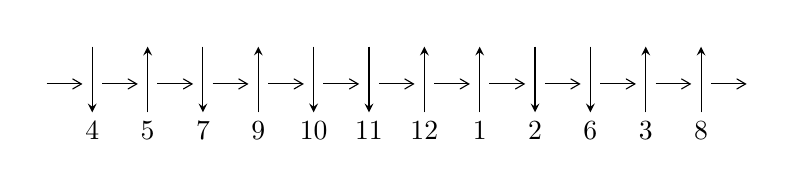
\begin{tikzpicture}[x=20pt, y=17pt]
	% nodes
	\node (C0) at (0, 0) {};
	\node (C1) at (1, 0) {};
	\node (C1U) at (1, +1) {};
	\node (C1D) at (1, -1) {4};

	\node (C2) at (2, 0) {};
	\node (C2U) at (2, +1) {};
	\node (C2D) at (2, -1) {5};

	\node (C3) at (3, 0) {};
	\node (C3U) at (3, +1) {};
	\node (C3D) at (3, -1) {7};

	\node (C4) at (4, 0) {};
	\node (C4U) at (4, +1) {};
	\node (C4D) at (4, -1) {9};

	\node (C5) at (5, 0) {};
	\node (C5U) at (5, +1) {};
	\node (C5D) at (5, -1) {10};

	\node (C6) at (6, 0) {};
	\node (C6U) at (6, +1) {};
	\node (C6D) at (6, -1) {11};

	\node (C7) at (7, 0) {};
	\node (C7U) at (7, +1) {};
	\node (C7D) at (7, -1) {12};

	\node (C8) at (8, 0) {};
	\node (C8U) at (8, +1) {};
	\node (C8D) at (8, -1) {1};

	\node (C9) at (9, 0) {};
	\node (C9U) at (9, +1) {};
	\node (C9D) at (9, -1) {2};

	\node (C10) at (10, 0) {};
	\node (C10U) at (10, +1) {};
	\node (C10D) at (10, -1) {6};

	\node (C11) at (11, 0) {};
	\node (C11U) at (11, +1) {};
	\node (C11D) at (11, -1) {3};

	\node (C12) at (12, 0) {};
	\node (C12U) at (12, +1) {};
	\node (C12D) at (12, -1) {8};
	\node (C13) at (13, 0) {};

	% arrows
	\draw[->,>={angle 60}]
	(C0) edge (C1) (C1) edge (C2) (C2) edge (C3) (C3) edge (C4) (C4) edge (C5) (C5) edge (C6) (C6) edge (C7) (C7) edge (C8) (C8) edge (C9) (C9) edge (C10) (C10) edge (C11) (C11) edge (C12) (C12) edge (C13) ;	\draw[->,>=stealth]
	(C1U) edge (C1D) (C2D) edge (C2U) (C3U) edge (C3D) (C4D) edge (C4U) (C5U) edge (C5D) (C6U) edge (C6D) (C7D) edge (C7U) (C8D) edge (C8U) (C9U) edge (C9D) (C10U) edge (C10D) (C11D) edge (C11U) (C12D) edge (C12U) ;
	\end{tikzpicture} \\
\hhline{~~} \\& 
\textbf{Solving Sequence} \\ \cline{2-2} 
 &
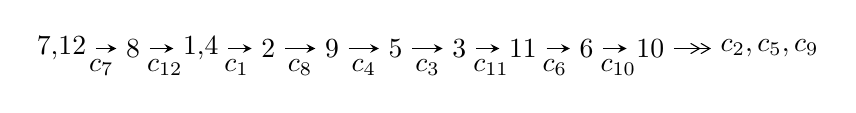
\begin{tikzpicture}[x=23pt, y=7pt]
	% node
	\node (A0) at (-1/8, 0) {7,12};
	\node (A1) at (1, 0) {8};
	\node (A2) at (33/16, 0) {1,4};
	\node (A3) at (25/8, 0) {2};
	\node (A4) at (33/8, 0) {9};
	\node (A5) at (41/8, 0) {5};
	\node (A6) at (49/8, 0) {3};
	\node (A7) at (57/8, 0) {11};
	\node (A8) at (65/8, 0) {6};
	\node (A9) at (73/8, 0) {10};
	\node (C1) at (1/2, -1) {$c_{7}$};
	\node (C2) at (3/2, -1) {$c_{12}$};
	\node (C3) at (21/8, -1) {$c_{1}$};
	\node (C4) at (29/8, -1) {$c_{8}$};
	\node (C5) at (37/8, -1) {$c_{4}$};
	\node (C6) at (45/8, -1) {$c_{3}$};
	\node (C7) at (53/8, -1) {$c_{11}$};
	\node (C8) at (61/8, -1) {$c_{6}$};
	\node (C9) at (69/8, -1) {$c_{10}$};
	\node (A10) at (11, 0) {$c_{2},c_{5},c_{9}$};

	% edge
	\draw[->,>=stealth]	
	(A0) edge (A1) (A1) edge (A2) (A2) edge (A3) (A3) edge (A4) (A4) edge (A5) (A5) edge (A6) (A6) edge (A7) (A7) edge (A8) (A8) edge (A9) ;
	\draw[->>,>={angle 60}]	
	(A9) edge (A10);
\end{tikzpicture} \\ 

\end{tabular} \\

\footnotetext{
The image of knot diagram is generated by the software ``\textbf{Draw programme}" developed by Andrew Bartholomew(\url{http://www.layer8.co.uk/maths/draw/index.htm\#Running-draw}), where we modified some parts for our purpose(\url{https://github.com/CATsTAILs/LinksPainter}).
}\phantom \\ \newline 
\centering \textbf{Ideals for irreducible components\footnotemark of $X_{\text{par}}$} 
 
\begin{align*}
I^u_{1}&=\langle 
9.81389\times10^{215} u^{101}-1.43564\times10^{216} u^{100}+\cdots+8.44851\times10^{215} b+1.19663\times10^{217},\\
\phantom{I^u_{1}}&\phantom{= \langle  }-2.45404\times10^{217} u^{101}+2.90155\times10^{217} u^{100}+\cdots+4.22426\times10^{216} a-2.42146\times10^{218},\\
\phantom{I^u_{1}}&\phantom{= \langle  }u^{102}- u^{101}+\cdots+18 u+1\rangle \\
I^u_{2}&=\langle 
u^{15}-9 u^{13}+u^{12}+33 u^{11}-6 u^{10}-61 u^9+11 u^8+54 u^7-2 u^6-13 u^5-11 u^4-5 u^3+6 u^2+b- u,\\
\phantom{I^u_{2}}&\phantom{= \langle  }5 u^{15}-340 u^{14}+\cdots+361 a-237,\\
\phantom{I^u_{2}}&\phantom{= \langle  }u^{16}- u^{15}-9 u^{14}+9 u^{13}+33 u^{12}-32 u^{11}-62 u^{10}+53 u^9+61 u^8-32 u^7-28 u^6-11 u^5+4 u^4+13 u^3+u+1\rangle \\
I^u_{3}&=\langle 
b-1,\;a+u+2,\;u^2+u-1\rangle \\
\\
\end{align*}
\raggedright * 3 irreducible components of $\dim_{\mathbb{C}}=0$, with total 120 representations.\\
\footnotetext{All coefficients of polynomials are rational numbers. But the coefficients are sometimes approximated in decimal forms when there is not enough margin.}
\newpage
\renewcommand{\arraystretch}{1}
\centering \section*{I. $I^u_{1}= \langle 9.81\times10^{215} u^{101}-1.44\times10^{216} u^{100}+\cdots+8.45\times10^{215} b+1.20\times10^{217},\;-2.45\times10^{217} u^{101}+2.90\times10^{217} u^{100}+\cdots+4.22\times10^{216} a-2.42\times10^{218},\;u^{102}- u^{101}+\cdots+18 u+1 \rangle$}
\flushleft \textbf{(i) Arc colorings}\\
\begin{tabular}{m{7pt} m{180pt} m{7pt} m{180pt} }
\flushright $a_{7}=$&$\begin{pmatrix}1\\0\end{pmatrix}$ \\
\flushright $a_{12}=$&$\begin{pmatrix}0\\u\end{pmatrix}$ \\
\flushright $a_{8}=$&$\begin{pmatrix}1\\- u^2\end{pmatrix}$ \\
\flushright $a_{1}=$&$\begin{pmatrix}u\\- u^3+u\end{pmatrix}$ \\
\flushright $a_{4}=$&$\begin{pmatrix}5.80939 u^{101}-6.86878 u^{100}+\cdots+523.205 u+57.3228\\-1.16161 u^{101}+1.69928 u^{100}+\cdots-146.794 u-14.1638\end{pmatrix}$ \\
\flushright $a_{2}=$&$\begin{pmatrix}17.1128 u^{101}-19.5202 u^{100}+\cdots+1275.28 u+124.279\\-2.65881 u^{101}+3.09872 u^{100}+\cdots-216.087 u-19.4356\end{pmatrix}$ \\
\flushright $a_{9}=$&$\begin{pmatrix}- u^2+1\\u^4-2 u^2\end{pmatrix}$ \\
\flushright $a_{5}=$&$\begin{pmatrix}4.60503 u^{101}-5.11479 u^{100}+\cdots+386.505 u+44.5732\\-1.25041 u^{101}+1.65858 u^{100}+\cdots-144.962 u-13.8921\end{pmatrix}$ \\
\flushright $a_{3}=$&$\begin{pmatrix}4.64778 u^{101}-5.16950 u^{100}+\cdots+376.411 u+43.1589\\-1.16161 u^{101}+1.69928 u^{100}+\cdots-146.794 u-14.1638\end{pmatrix}$ \\
\flushright $a_{11}=$&$\begin{pmatrix}9.69143 u^{101}-11.7940 u^{100}+\cdots+697.904 u+71.4195\\-2.46283 u^{101}+2.72548 u^{100}+\cdots-193.856 u-17.8946\end{pmatrix}$ \\
\flushright $a_{6}=$&$\begin{pmatrix}21.5584 u^{101}-23.9838 u^{100}+\cdots+1850.82 u+175.409\\-1.80773 u^{101}+1.92185 u^{100}+\cdots-143.234 u-14.0282\end{pmatrix}$ \\
\flushright $a_{10}=$&$\begin{pmatrix}-25.0084 u^{101}+29.3750 u^{100}+\cdots-1856.25 u-168.712\\2.27979 u^{101}-2.77364 u^{100}+\cdots+167.806 u+16.0557\end{pmatrix}$\\&\end{tabular}
\flushleft \textbf{(ii) Obstruction class $= -1$}\\~\\
\flushleft \textbf{(iii) Cusp Shapes $= -14.2614 u^{101}+16.1606 u^{100}+\cdots-745.362 u-63.3257$}\\~\\
\newpage\renewcommand{\arraystretch}{1}
\flushleft \textbf{(iv) u-Polynomials at the component}\newline \\
\begin{tabular}{m{50pt}|m{274pt}}
Crossings & \hspace{64pt}u-Polynomials at each crossing \\
\hline $$\begin{aligned}c_{1}\end{aligned}$$&$\begin{aligned}
&u^{102}+8 u^{101}+\cdots+2562 u-279
\end{aligned}$\\
\hline $$\begin{aligned}c_{2}\end{aligned}$$&$\begin{aligned}
&u^{102}-8 u^{101}+\cdots-2562 u-279
\end{aligned}$\\
\hline $$\begin{aligned}c_{3}\end{aligned}$$&$\begin{aligned}
&u^{102}+3 u^{101}+\cdots+27 u-1
\end{aligned}$\\
\hline $$\begin{aligned}c_{4}\end{aligned}$$&$\begin{aligned}
&u^{102}- u^{101}+\cdots+1378 u+1357
\end{aligned}$\\
\hline $$\begin{aligned}c_{5},c_{6},c_{10}\end{aligned}$$&$\begin{aligned}
&u^{102}- u^{101}+\cdots+18 u+1
\end{aligned}$\\
\hline $$\begin{aligned}c_{7},c_{8},c_{12}\end{aligned}$$&$\begin{aligned}
&u^{102}+u^{101}+\cdots-18 u+1
\end{aligned}$\\
\hline $$\begin{aligned}c_{9}\end{aligned}$$&$\begin{aligned}
&u^{102}+u^{101}+\cdots-1378 u+1357
\end{aligned}$\\
\hline $$\begin{aligned}c_{11}\end{aligned}$$&$\begin{aligned}
&u^{102}-3 u^{101}+\cdots-27 u-1
\end{aligned}$\\
\hline
\end{tabular}\\~\\
\newpage\renewcommand{\arraystretch}{1}
\flushleft \textbf{(v) Riley Polynomials at the component}\newline \\
\begin{tabular}{m{50pt}|m{274pt}}
Crossings & \hspace{64pt}Riley Polynomials at each crossing \\
\hline $$\begin{aligned}c_{1},c_{2}\end{aligned}$$&$\begin{aligned}
&y^{102}+18 y^{101}+\cdots+642168 y+77841
\end{aligned}$\\
\hline $$\begin{aligned}c_{3},c_{11}\end{aligned}$$&$\begin{aligned}
&y^{102}-5 y^{101}+\cdots-1355 y+1
\end{aligned}$\\
\hline $$\begin{aligned}c_{4},c_{9}\end{aligned}$$&$\begin{aligned}
&y^{102}-33 y^{101}+\cdots-92622476 y+1841449
\end{aligned}$\\
\hline $$\begin{aligned}c_{5},c_{6},c_{7}\\c_{8},c_{10},c_{12}\end{aligned}$$&$\begin{aligned}
&y^{102}-109 y^{101}+\cdots-154 y+1
\end{aligned}$\\
\hline
\end{tabular}\\~\\
\newpage\flushleft \textbf{(vi) Complex Volumes and Cusp Shapes}
$$\begin{array}{c|c|c}  
\text{Solutions to }I^u_{1}& \I (\text{vol} + \sqrt{-1}CS) & \text{Cusp shape}\\
 \hline 
\begin{aligned}
u &= -0.421881 + 0.913460 I \\
a &= -0.165545 - 0.490628 I \\
b &= \phantom{-}0.888810 - 0.537019 I\end{aligned}
 & -8.03164 + 7.68352 I & \phantom{-0.000000 } 0 \\ \hline\begin{aligned}
u &= -0.421881 - 0.913460 I \\
a &= -0.165545 + 0.490628 I \\
b &= \phantom{-}0.888810 + 0.537019 I\end{aligned}
 & -8.03164 - 7.68352 I & \phantom{-0.000000 } 0 \\ \hline\begin{aligned}
u &= \phantom{-}0.948769 + 0.365737 I \\
a &= \phantom{-}0.663232 + 0.274203 I \\
b &= \phantom{-}1.233530 - 0.266394 I\end{aligned}
 & -4.88209 - 0.50422 I & \phantom{-0.000000 } 0 \\ \hline\begin{aligned}
u &= \phantom{-}0.948769 - 0.365737 I \\
a &= \phantom{-}0.663232 - 0.274203 I \\
b &= \phantom{-}1.233530 + 0.266394 I\end{aligned}
 & -4.88209 + 0.50422 I & \phantom{-0.000000 } 0 \\ \hline\begin{aligned}
u &= -0.649076 + 0.789280 I \\
a &= \phantom{-}0.353140 - 0.770907 I \\
b &= \phantom{-}1.18870 + 0.83480 I\end{aligned}
 & -7.3328 - 13.2263 I & \phantom{-0.000000 } 0 \\ \hline\begin{aligned}
u &= -0.649076 - 0.789280 I \\
a &= \phantom{-}0.353140 + 0.770907 I \\
b &= \phantom{-}1.18870 - 0.83480 I\end{aligned}
 & -7.3328 + 13.2263 I & \phantom{-0.000000 } 0 \\ \hline\begin{aligned}
u &= \phantom{-}0.656934 + 0.801294 I \\
a &= -0.230937 - 0.577852 I \\
b &= -0.860693 + 0.757017 I\end{aligned}
 & \phantom{-0.000000 -}9.25295 I & \phantom{-0.000000 } 0 \\ \hline\begin{aligned}
u &= \phantom{-}0.656934 - 0.801294 I \\
a &= -0.230937 + 0.577852 I \\
b &= -0.860693 - 0.757017 I\end{aligned}
 & \phantom{-0.000000 } -9.25295 I & \phantom{-0.000000 } 0 \\ \hline\begin{aligned}
u &= -0.618166 + 0.738762 I \\
a &= -0.455893 + 0.460022 I \\
b &= -0.586392 - 0.519509 I\end{aligned}
 & \phantom{-}1.45177 - 2.24448 I & \phantom{-0.000000 } 0 \\ \hline\begin{aligned}
u &= -0.618166 - 0.738762 I \\
a &= -0.455893 - 0.460022 I \\
b &= -0.586392 + 0.519509 I\end{aligned}
 & \phantom{-}1.45177 + 2.24448 I & \phantom{-0.000000 } 0\\
 \hline 
 \end{array}$$\newpage$$\begin{array}{c|c|c}  
\text{Solutions to }I^u_{1}& \I (\text{vol} + \sqrt{-1}CS) & \text{Cusp shape}\\
 \hline 
\begin{aligned}
u &= \phantom{-}0.748254 + 0.536631 I \\
a &= \phantom{-}1.006120 - 0.725807 I \\
b &= -0.816259 - 0.391671 I\end{aligned}
 & -7.39412 - 1.87601 I & \phantom{-0.000000 } 0 \\ \hline\begin{aligned}
u &= \phantom{-}0.748254 - 0.536631 I \\
a &= \phantom{-}1.006120 + 0.725807 I \\
b &= -0.816259 + 0.391671 I\end{aligned}
 & -7.39412 + 1.87601 I & \phantom{-0.000000 } 0 \\ \hline\begin{aligned}
u &= \phantom{-}0.356069 + 1.033270 I \\
a &= \phantom{-}0.118651 - 0.235636 I \\
b &= -0.441341 - 0.229273 I\end{aligned}
 & -0.84908 - 3.47127 I & \phantom{-0.000000 } 0 \\ \hline\begin{aligned}
u &= \phantom{-}0.356069 - 1.033270 I \\
a &= \phantom{-}0.118651 + 0.235636 I \\
b &= -0.441341 + 0.229273 I\end{aligned}
 & -0.84908 + 3.47127 I & \phantom{-0.000000 } 0 \\ \hline\begin{aligned}
u &= -0.631769 + 0.896852 I \\
a &= \phantom{-}0.037064 - 0.290429 I \\
b &= \phantom{-}0.365478 + 0.498966 I\end{aligned}
 & \phantom{-}0.84908 - 3.47127 I & \phantom{-0.000000 } 0 \\ \hline\begin{aligned}
u &= -0.631769 - 0.896852 I \\
a &= \phantom{-}0.037064 + 0.290429 I \\
b &= \phantom{-}0.365478 - 0.498966 I\end{aligned}
 & \phantom{-}0.84908 + 3.47127 I & \phantom{-0.000000 } 0 \\ \hline\begin{aligned}
u &= -0.847496 + 0.274573 I \\
a &= -0.446501 + 0.051731 I \\
b &= -0.886146 - 0.010622 I\end{aligned}
 & \phantom{-}0.652997 + 0.202759 I & \phantom{-0.000000 } 0 \\ \hline\begin{aligned}
u &= -0.847496 - 0.274573 I \\
a &= -0.446501 - 0.051731 I \\
b &= -0.886146 + 0.010622 I\end{aligned}
 & \phantom{-}0.652997 - 0.202759 I & \phantom{-0.000000 } 0 \\ \hline\begin{aligned}
u &= \phantom{-}0.446889 + 0.764035 I \\
a &= \phantom{-}0.953721 + 0.634503 I \\
b &= \phantom{-}0.917901 - 0.731514 I\end{aligned}
 & -3.55803 + 4.98722 I & \phantom{-0.000000 } 0 \\ \hline\begin{aligned}
u &= \phantom{-}0.446889 - 0.764035 I \\
a &= \phantom{-}0.953721 - 0.634503 I \\
b &= \phantom{-}0.917901 + 0.731514 I\end{aligned}
 & -3.55803 - 4.98722 I & \phantom{-0.000000 } 0\\
 \hline 
 \end{array}$$\newpage$$\begin{array}{c|c|c}  
\text{Solutions to }I^u_{1}& \I (\text{vol} + \sqrt{-1}CS) & \text{Cusp shape}\\
 \hline 
\begin{aligned}
u &= \phantom{-}0.607479 + 0.536834 I \\
a &= -0.057997 + 0.146408 I \\
b &= \phantom{-}0.625451 + 0.753642 I\end{aligned}
 & -2.87163 - 0.43109 I & \phantom{-0.000000 } 0 \\ \hline\begin{aligned}
u &= \phantom{-}0.607479 - 0.536834 I \\
a &= -0.057997 - 0.146408 I \\
b &= \phantom{-}0.625451 - 0.753642 I\end{aligned}
 & -2.87163 + 0.43109 I & \phantom{-0.000000 } 0 \\ \hline\begin{aligned}
u &= \phantom{-}1.243250 + 0.067945 I \\
a &= \phantom{-}0.863393 - 0.902732 I \\
b &= -0.183056 - 0.072866 I\end{aligned}
 & -3.85916 + 1.48032 I & \phantom{-0.000000 } 0 \\ \hline\begin{aligned}
u &= \phantom{-}1.243250 - 0.067945 I \\
a &= \phantom{-}0.863393 + 0.902732 I \\
b &= -0.183056 + 0.072866 I\end{aligned}
 & -3.85916 - 1.48032 I & \phantom{-0.000000 } 0 \\ \hline\begin{aligned}
u &= -0.536711 + 0.504007 I \\
a &= -0.351562 + 1.204950 I \\
b &= -1.33435 - 1.00611 I\end{aligned}
 & -7.91386 - 3.73886 I & \phantom{-0.000000 } 0 \\ \hline\begin{aligned}
u &= -0.536711 - 0.504007 I \\
a &= -0.351562 - 1.204950 I \\
b &= -1.33435 + 1.00611 I\end{aligned}
 & -7.91386 + 3.73886 I & \phantom{-0.000000 } 0 \\ \hline\begin{aligned}
u &= \phantom{-}0.332736 + 0.635981 I \\
a &= -0.486881 - 0.278645 I \\
b &= -1.24108 + 0.82202 I\end{aligned}
 & -8.60735 + 5.94490 I & \phantom{-0.000000 } 0 \\ \hline\begin{aligned}
u &= \phantom{-}0.332736 - 0.635981 I \\
a &= -0.486881 + 0.278645 I \\
b &= -1.24108 - 0.82202 I\end{aligned}
 & -8.60735 - 5.94490 I & \phantom{-0.000000 } 0 \\ \hline\begin{aligned}
u &= -0.166338 + 0.666357 I \\
a &= \phantom{-}0.252426 - 0.088045 I \\
b &= \phantom{-}0.688253 + 0.733228 I\end{aligned}
 & -1.45177 - 2.24448 I & -7.42940 + 6.53557 I \\ \hline\begin{aligned}
u &= -0.166338 - 0.666357 I \\
a &= \phantom{-}0.252426 + 0.088045 I \\
b &= \phantom{-}0.688253 - 0.733228 I\end{aligned}
 & -1.45177 + 2.24448 I & -7.42940 - 6.53557 I\\
 \hline 
 \end{array}$$\newpage$$\begin{array}{c|c|c}  
\text{Solutions to }I^u_{1}& \I (\text{vol} + \sqrt{-1}CS) & \text{Cusp shape}\\
 \hline 
\begin{aligned}
u &= \phantom{-}0.479515 + 0.488023 I \\
a &= \phantom{-}0.279138 + 1.179520 I \\
b &= \phantom{-}0.885725 - 0.779306 I\end{aligned}
 & -1.44911 + 3.19144 I & -7.35679 - 8.71973 I \\ \hline\begin{aligned}
u &= \phantom{-}0.479515 - 0.488023 I \\
a &= \phantom{-}0.279138 - 1.179520 I \\
b &= \phantom{-}0.885725 + 0.779306 I\end{aligned}
 & -1.44911 - 3.19144 I & -7.35679 + 8.71973 I \\ \hline\begin{aligned}
u &= -1.335720 + 0.108681 I \\
a &= -0.37231 + 1.37405 I \\
b &= -0.138461 - 0.851390 I\end{aligned}
 & \phantom{-}2.87163 - 0.43109 I & \phantom{-0.000000 } 0 \\ \hline\begin{aligned}
u &= -1.335720 - 0.108681 I \\
a &= -0.37231 - 1.37405 I \\
b &= -0.138461 + 0.851390 I\end{aligned}
 & \phantom{-}2.87163 + 0.43109 I & \phantom{-0.000000 } 0 \\ \hline\begin{aligned}
u &= \phantom{-}0.159323 + 0.633172 I \\
a &= \phantom{-}1.12688 + 1.85019 I \\
b &= \phantom{-}0.711101 + 0.356367 I\end{aligned}
 & -7.28113 + 4.19641 I & -7.17543 - 4.77818 I \\ \hline\begin{aligned}
u &= \phantom{-}0.159323 - 0.633172 I \\
a &= \phantom{-}1.12688 - 1.85019 I \\
b &= \phantom{-}0.711101 - 0.356367 I\end{aligned}
 & -7.28113 - 4.19641 I & -7.17543 + 4.77818 I \\ \hline\begin{aligned}
u &= -0.264474 + 0.551378 I \\
a &= -0.72511 + 1.64636 I \\
b &= -0.569908 - 0.161854 I\end{aligned}
 & -1.10064 - 3.42771 I & -7.99632 + 9.02699 I \\ \hline\begin{aligned}
u &= -0.264474 - 0.551378 I \\
a &= -0.72511 - 1.64636 I \\
b &= -0.569908 + 0.161854 I\end{aligned}
 & -1.10064 + 3.42771 I & -7.99632 - 9.02699 I \\ \hline\begin{aligned}
u &= -1.388920 + 0.144019 I \\
a &= -0.23998 - 1.64481 I \\
b &= \phantom{-}0.1004980 - 0.0409276 I\end{aligned}
 & -2.44020 - 6.79345 I & \phantom{-0.000000 } 0 \\ \hline\begin{aligned}
u &= -1.388920 - 0.144019 I \\
a &= -0.23998 + 1.64481 I \\
b &= \phantom{-}0.1004980 + 0.0409276 I\end{aligned}
 & -2.44020 + 6.79345 I & \phantom{-0.000000 } 0\\
 \hline 
 \end{array}$$\newpage$$\begin{array}{c|c|c}  
\text{Solutions to }I^u_{1}& \I (\text{vol} + \sqrt{-1}CS) & \text{Cusp shape}\\
 \hline 
\begin{aligned}
u &= -0.595566 + 0.056430 I \\
a &= -1.275670 + 0.429355 I \\
b &= -0.102020 - 0.301000 I\end{aligned}
 & \phantom{-}1.42393 - 0.14814 I & \phantom{-}6.94586 - 0.46279 I \\ \hline\begin{aligned}
u &= -0.595566 - 0.056430 I \\
a &= -1.275670 - 0.429355 I \\
b &= -0.102020 + 0.301000 I\end{aligned}
 & \phantom{-}1.42393 + 0.14814 I & \phantom{-}6.94586 + 0.46279 I \\ \hline\begin{aligned}
u &= -1.40670\phantom{ +0.000000I} \\
a &= -0.190717\phantom{ +0.000000I} \\
b &= -1.36954\phantom{ +0.000000I}\end{aligned}
 & -3.91844\phantom{ +0.000000I} & \phantom{-0.000000 } 0 \\ \hline\begin{aligned}
u &= \phantom{-}1.403230 + 0.157306 I \\
a &= -0.20679 + 1.82905 I \\
b &= \phantom{-}0.91053 - 1.38663 I\end{aligned}
 & \phantom{-}3.55803 + 4.98722 I & \phantom{-0.000000 } 0 \\ \hline\begin{aligned}
u &= \phantom{-}1.403230 - 0.157306 I \\
a &= -0.20679 - 1.82905 I \\
b &= \phantom{-}0.91053 + 1.38663 I\end{aligned}
 & \phantom{-}3.55803 - 4.98722 I & \phantom{-0.000000 } 0 \\ \hline\begin{aligned}
u &= -0.530263 + 0.189652 I \\
a &= \phantom{-}0.499941 + 0.711171 I \\
b &= \phantom{-}0.12126 - 1.59467 I\end{aligned}
 & -4.46231 - 5.76178 I & \phantom{-}1.80073 + 7.63380 I \\ \hline\begin{aligned}
u &= -0.530263 - 0.189652 I \\
a &= \phantom{-}0.499941 - 0.711171 I \\
b &= \phantom{-}0.12126 + 1.59467 I\end{aligned}
 & -4.46231 + 5.76178 I & \phantom{-}1.80073 - 7.63380 I \\ \hline\begin{aligned}
u &= -0.323849 + 0.452126 I \\
a &= \phantom{-}0.87936 + 1.56567 I \\
b &= -1.076990 + 0.414157 I\end{aligned}
 & -8.42239 + 0.35931 I & -8.15948 + 0.80270 I \\ \hline\begin{aligned}
u &= -0.323849 - 0.452126 I \\
a &= \phantom{-}0.87936 - 1.56567 I \\
b &= -1.076990 - 0.414157 I\end{aligned}
 & -8.42239 - 0.35931 I & -8.15948 - 0.80270 I \\ \hline\begin{aligned}
u &= \phantom{-}1.44559 + 0.13953 I \\
a &= \phantom{-}0.13946 - 1.68727 I \\
b &= -0.161842 + 0.586300 I\end{aligned}
 & \phantom{-}4.46231 + 5.76178 I & \phantom{-0.000000 } 0\\
 \hline 
 \end{array}$$\newpage$$\begin{array}{c|c|c}  
\text{Solutions to }I^u_{1}& \I (\text{vol} + \sqrt{-1}CS) & \text{Cusp shape}\\
 \hline 
\begin{aligned}
u &= \phantom{-}1.44559 - 0.13953 I \\
a &= \phantom{-}0.13946 + 1.68727 I \\
b &= -0.161842 - 0.586300 I\end{aligned}
 & \phantom{-}4.46231 - 5.76178 I & \phantom{-0.000000 } 0 \\ \hline\begin{aligned}
u &= \phantom{-}0.466187 + 0.285491 I \\
a &= -0.684856 + 0.412840 I \\
b &= \phantom{-}0.813263 + 0.154187 I\end{aligned}
 & -1.42393 - 0.14814 I & -6.94586 - 0.46279 I \\ \hline\begin{aligned}
u &= \phantom{-}0.466187 - 0.285491 I \\
a &= -0.684856 - 0.412840 I \\
b &= \phantom{-}0.813263 - 0.154187 I\end{aligned}
 & -1.42393 + 0.14814 I & -6.94586 + 0.46279 I \\ \hline\begin{aligned}
u &= \phantom{-}1.45431 + 0.02048 I \\
a &= -0.951292 - 0.896201 I \\
b &= \phantom{-}1.79673 + 0.70112 I\end{aligned}
 & \phantom{-}4.88209 + 0.50422 I & \phantom{-0.000000 } 0 \\ \hline\begin{aligned}
u &= \phantom{-}1.45431 - 0.02048 I \\
a &= -0.951292 + 0.896201 I \\
b &= \phantom{-}1.79673 - 0.70112 I\end{aligned}
 & \phantom{-}4.88209 - 0.50422 I & \phantom{-0.000000 } 0 \\ \hline\begin{aligned}
u &= -1.44798 + 0.18036 I \\
a &= \phantom{-}0.72702 + 1.82534 I \\
b &= -1.57595 - 1.31600 I\end{aligned}
 & -2.86058 - 8.79148 I & \phantom{-0.000000 } 0 \\ \hline\begin{aligned}
u &= -1.44798 - 0.18036 I \\
a &= \phantom{-}0.72702 - 1.82534 I \\
b &= -1.57595 + 1.31600 I\end{aligned}
 & -2.86058 + 8.79148 I & \phantom{-0.000000 } 0 \\ \hline\begin{aligned}
u &= -1.48460 + 0.05083 I \\
a &= \phantom{-}0.63408 - 1.77146 I \\
b &= -1.10430 + 1.51531 I\end{aligned}
 & \phantom{-}7.28113 - 4.19641 I & \phantom{-0.000000 } 0 \\ \hline\begin{aligned}
u &= -1.48460 - 0.05083 I \\
a &= \phantom{-}0.63408 + 1.77146 I \\
b &= -1.10430 - 1.51531 I\end{aligned}
 & \phantom{-}7.28113 + 4.19641 I & \phantom{-0.000000 } 0 \\ \hline\begin{aligned}
u &= \phantom{-}1.48976 + 0.04878 I \\
a &= -0.05888 - 2.10123 I \\
b &= -0.93265 + 1.08671 I\end{aligned}
 & \phantom{-}1.00808 + 6.07571 I & \phantom{-0.000000 } 0\\
 \hline 
 \end{array}$$\newpage$$\begin{array}{c|c|c}  
\text{Solutions to }I^u_{1}& \I (\text{vol} + \sqrt{-1}CS) & \text{Cusp shape}\\
 \hline 
\begin{aligned}
u &= \phantom{-}1.48976 - 0.04878 I \\
a &= -0.05888 + 2.10123 I \\
b &= -0.93265 - 1.08671 I\end{aligned}
 & \phantom{-}1.00808 - 6.07571 I & \phantom{-0.000000 } 0 \\ \hline\begin{aligned}
u &= -1.49523 + 0.07916 I \\
a &= -0.79260 + 1.22174 I \\
b &= \phantom{-}0.91211 - 1.16668 I\end{aligned}
 & \phantom{-}3.85916 - 1.48032 I & \phantom{-0.000000 } 0 \\ \hline\begin{aligned}
u &= -1.49523 - 0.07916 I \\
a &= -0.79260 - 1.22174 I \\
b &= \phantom{-}0.91211 + 1.16668 I\end{aligned}
 & \phantom{-}3.85916 + 1.48032 I & \phantom{-0.000000 } 0 \\ \hline\begin{aligned}
u &= -1.49922 + 0.03734 I \\
a &= \phantom{-}0.10155 - 1.60495 I \\
b &= \phantom{-}0.804629 + 0.956431 I\end{aligned}
 & \phantom{-}7.91386 - 3.73886 I & \phantom{-0.000000 } 0 \\ \hline\begin{aligned}
u &= -1.49922 - 0.03734 I \\
a &= \phantom{-}0.10155 + 1.60495 I \\
b &= \phantom{-}0.804629 - 0.956431 I\end{aligned}
 & \phantom{-}7.91386 + 3.73886 I & \phantom{-0.000000 } 0 \\ \hline\begin{aligned}
u &= \phantom{-}1.52152 + 0.00958 I \\
a &= \phantom{-}0.121602 - 0.998252 I \\
b &= -0.831129 + 0.730519 I\end{aligned}
 & \phantom{-}8.42239 + 0.35931 I & \phantom{-0.000000 } 0 \\ \hline\begin{aligned}
u &= \phantom{-}1.52152 - 0.00958 I \\
a &= \phantom{-}0.121602 + 0.998252 I \\
b &= -0.831129 - 0.730519 I\end{aligned}
 & \phantom{-}8.42239 - 0.35931 I & \phantom{-0.000000 } 0 \\ \hline\begin{aligned}
u &= \phantom{-}1.52779 + 0.07140 I \\
a &= -0.37212 - 2.35107 I \\
b &= \phantom{-}0.43650 + 2.32127 I\end{aligned}
 & \phantom{-}2.44020 + 6.79345 I & \phantom{-0.000000 } 0 \\ \hline\begin{aligned}
u &= \phantom{-}1.52779 - 0.07140 I \\
a &= -0.37212 + 2.35107 I \\
b &= \phantom{-}0.43650 - 2.32127 I\end{aligned}
 & \phantom{-}2.44020 - 6.79345 I & \phantom{-0.000000 } 0 \\ \hline\begin{aligned}
u &= -1.52325 + 0.14078 I \\
a &= -0.43026 - 2.00109 I \\
b &= \phantom{-}0.86769 + 1.39894 I\end{aligned}
 & \phantom{-}5.22562 - 5.43260 I & \phantom{-0.000000 } 0\\
 \hline 
 \end{array}$$\newpage$$\begin{array}{c|c|c}  
\text{Solutions to }I^u_{1}& \I (\text{vol} + \sqrt{-1}CS) & \text{Cusp shape}\\
 \hline 
\begin{aligned}
u &= -1.52325 - 0.14078 I \\
a &= -0.43026 + 2.00109 I \\
b &= \phantom{-}0.86769 - 1.39894 I\end{aligned}
 & \phantom{-}5.22562 + 5.43260 I & \phantom{-0.000000 } 0 \\ \hline\begin{aligned}
u &= -1.51654 + 0.27355 I \\
a &= \phantom{-}0.02065 - 1.54952 I \\
b &= \phantom{-}1.13737 + 0.89063 I\end{aligned}
 & \phantom{-}2.86058 - 8.79148 I & \phantom{-0.000000 } 0 \\ \hline\begin{aligned}
u &= -1.51654 - 0.27355 I \\
a &= \phantom{-}0.02065 + 1.54952 I \\
b &= \phantom{-}1.13737 - 0.89063 I\end{aligned}
 & \phantom{-}2.86058 + 8.79148 I & \phantom{-0.000000 } 0 \\ \hline\begin{aligned}
u &= \phantom{-}1.53675 + 0.14550 I \\
a &= \phantom{-}0.75979 - 2.20368 I \\
b &= -1.42765 + 1.55977 I\end{aligned}
 & -1.00808 + 6.07571 I & \phantom{-0.000000 } 0 \\ \hline\begin{aligned}
u &= \phantom{-}1.53675 - 0.14550 I \\
a &= \phantom{-}0.75979 + 2.20368 I \\
b &= -1.42765 - 1.55977 I\end{aligned}
 & -1.00808 - 6.07571 I & \phantom{-0.000000 } 0 \\ \hline\begin{aligned}
u &= -1.49251 + 0.43030 I \\
a &= -0.346839 + 0.639465 I \\
b &= \phantom{-}0.067986 - 0.620504 I\end{aligned}
 & \phantom{-}2.28760 - 2.26927 I & \phantom{-0.000000 } 0 \\ \hline\begin{aligned}
u &= -1.49251 - 0.43030 I \\
a &= -0.346839 - 0.639465 I \\
b &= \phantom{-}0.067986 + 0.620504 I\end{aligned}
 & \phantom{-}2.28760 + 2.26927 I & \phantom{-0.000000 } 0 \\ \hline\begin{aligned}
u &= \phantom{-}0.434805 + 0.097618 I \\
a &= \phantom{-}1.95914 + 2.03130 I \\
b &= \phantom{-}0.363256 - 0.760387 I\end{aligned}
 & \phantom{-}1.44911 + 3.19144 I & \phantom{-}7.35679 - 8.71973 I \\ \hline\begin{aligned}
u &= \phantom{-}0.434805 - 0.097618 I \\
a &= \phantom{-}1.95914 - 2.03130 I \\
b &= \phantom{-}0.363256 + 0.760387 I\end{aligned}
 & \phantom{-}1.44911 - 3.19144 I & \phantom{-}7.35679 + 8.71973 I \\ \hline\begin{aligned}
u &= \phantom{-}1.56268\phantom{ +0.000000I} \\
a &= \phantom{-}0.587667\phantom{ +0.000000I} \\
b &= -1.29423\phantom{ +0.000000I}\end{aligned}
 & \phantom{-}8.57239\phantom{ +0.000000I} & \phantom{-0.000000 } 0\\
 \hline 
 \end{array}$$\newpage$$\begin{array}{c|c|c}  
\text{Solutions to }I^u_{1}& \I (\text{vol} + \sqrt{-1}CS) & \text{Cusp shape}\\
 \hline 
\begin{aligned}
u &= \phantom{-}1.56445 + 0.25318 I \\
a &= \phantom{-}0.064615 - 1.305070 I \\
b &= -0.920531 + 0.918148 I\end{aligned}
 & \phantom{-}8.60735 + 5.94490 I & \phantom{-0.000000 } 0 \\ \hline\begin{aligned}
u &= \phantom{-}1.56445 - 0.25318 I \\
a &= \phantom{-}0.064615 + 1.305070 I \\
b &= -0.920531 - 0.918148 I\end{aligned}
 & \phantom{-}8.60735 - 5.94490 I & \phantom{-0.000000 } 0 \\ \hline\begin{aligned}
u &= \phantom{-}1.42824 + 0.69356 I \\
a &= -0.198797 + 0.184560 I \\
b &= \phantom{-}0.408032 + 0.148288 I\end{aligned}
 & -2.28760 - 2.26927 I & \phantom{-0.000000 } 0 \\ \hline\begin{aligned}
u &= \phantom{-}1.42824 - 0.69356 I \\
a &= -0.198797 - 0.184560 I \\
b &= \phantom{-}0.408032 - 0.148288 I\end{aligned}
 & -2.28760 + 2.26927 I & \phantom{-0.000000 } 0 \\ \hline\begin{aligned}
u &= \phantom{-}1.57263 + 0.28115 I \\
a &= -0.026754 + 1.327210 I \\
b &= \phantom{-}0.633582 - 1.094220 I\end{aligned}
 & \phantom{-}8.03164 + 7.68352 I & \phantom{-0.000000 } 0 \\ \hline\begin{aligned}
u &= \phantom{-}1.57263 - 0.28115 I \\
a &= -0.026754 - 1.327210 I \\
b &= \phantom{-}0.633582 + 1.094220 I\end{aligned}
 & \phantom{-}8.03164 - 7.68352 I & \phantom{-0.000000 } 0 \\ \hline\begin{aligned}
u &= -1.59918\phantom{ +0.000000I} \\
a &= -1.33841\phantom{ +0.000000I} \\
b &= \phantom{-}2.19481\phantom{ +0.000000I}\end{aligned}
 & \phantom{-}3.91844\phantom{ +0.000000I} & \phantom{-0.000000 } 0 \\ \hline\begin{aligned}
u &= -1.58178 + 0.26953 I \\
a &= \phantom{-}0.23352 + 1.56390 I \\
b &= -1.05120 - 1.17547 I\end{aligned}
 & \phantom{-}7.3328 - 13.2263 I & \phantom{-0.000000 } 0 \\ \hline\begin{aligned}
u &= -1.58178 - 0.26953 I \\
a &= \phantom{-}0.23352 - 1.56390 I \\
b &= -1.05120 + 1.17547 I\end{aligned}
 & \phantom{-}7.3328 + 13.2263 I & \phantom{-0.000000 } 0 \\ \hline\begin{aligned}
u &= \phantom{-}1.58356 + 0.26771 I \\
a &= -0.40968 + 1.69637 I \\
b &= \phantom{-}1.36740 - 1.13901 I\end{aligned}
 & \phantom{-0.000000 -}17.1602 I & \phantom{-0.000000 } 0\\
 \hline 
 \end{array}$$\newpage$$\begin{array}{c|c|c}  
\text{Solutions to }I^u_{1}& \I (\text{vol} + \sqrt{-1}CS) & \text{Cusp shape}\\
 \hline 
\begin{aligned}
u &= \phantom{-}1.58356 - 0.26771 I \\
a &= -0.40968 - 1.69637 I \\
b &= \phantom{-}1.36740 + 1.13901 I\end{aligned}
 & \phantom{-0.000000 } -17.1602 I & \phantom{-0.000000 } 0 \\ \hline\begin{aligned}
u &= \phantom{-}0.356649 + 0.156360 I \\
a &= -1.03119 + 1.31362 I \\
b &= -0.476026 - 1.106660 I\end{aligned}
 & \phantom{-}1.10064 + 3.42771 I & \phantom{-}7.99632 - 9.02699 I \\ \hline\begin{aligned}
u &= \phantom{-}0.356649 - 0.156360 I \\
a &= -1.03119 - 1.31362 I \\
b &= -0.476026 + 1.106660 I\end{aligned}
 & \phantom{-}1.10064 - 3.42771 I & \phantom{-}7.99632 + 9.02699 I \\ \hline\begin{aligned}
u &= -0.350648 + 0.105043 I \\
a &= -2.78594 + 3.95960 I \\
b &= -0.581556 - 0.978801 I\end{aligned}
 & -5.22562 - 5.43260 I & \phantom{-}6.43384 + 6.15958 I \\ \hline\begin{aligned}
u &= -0.350648 - 0.105043 I \\
a &= -2.78594 - 3.95960 I \\
b &= -0.581556 + 0.978801 I\end{aligned}
 & -5.22562 + 5.43260 I & \phantom{-}6.43384 - 6.15958 I \\ \hline\begin{aligned}
u &= -1.64265\phantom{ +0.000000I} \\
a &= \phantom{-}0.643909\phantom{ +0.000000I} \\
b &= -0.0289151\phantom{ +0.000000I}\end{aligned}
 & \phantom{-}1.46197\phantom{ +0.000000I} & \phantom{-0.000000 } 0 \\ \hline\begin{aligned}
u &= -1.64130 + 0.22779 I \\
a &= -0.221317 - 0.900678 I \\
b &= \phantom{-}0.741738 + 0.734271 I\end{aligned}
 & \phantom{-}7.39412 - 1.87601 I & \phantom{-0.000000 } 0 \\ \hline\begin{aligned}
u &= -1.64130 - 0.22779 I \\
a &= -0.221317 + 0.900678 I \\
b &= \phantom{-}0.741738 - 0.734271 I\end{aligned}
 & \phantom{-}7.39412 + 1.87601 I & \phantom{-0.000000 } 0 \\ \hline\begin{aligned}
u &= \phantom{-}1.67186\phantom{ +0.000000I} \\
a &= \phantom{-}0.992925\phantom{ +0.000000I} \\
b &= -1.01022\phantom{ +0.000000I}\end{aligned}
 & -1.46197\phantom{ +0.000000I} & \phantom{-0.000000 } 0 \\ \hline\begin{aligned}
u &= -0.147584 + 0.068672 I \\
a &= \phantom{-}3.79006 + 2.75652 I \\
b &= \phantom{-}1.118130 - 0.400748 I\end{aligned}
 & -0.652997 - 0.202759 I & -7.20656 + 6.25888 I\\
 \hline 
 \end{array}$$\newpage$$\begin{array}{c|c|c}  
\text{Solutions to }I^u_{1}& \I (\text{vol} + \sqrt{-1}CS) & \text{Cusp shape}\\
 \hline 
\begin{aligned}
u &= -0.147584 - 0.068672 I \\
a &= \phantom{-}3.79006 - 2.75652 I \\
b &= \phantom{-}1.118130 + 0.400748 I\end{aligned}
 & -0.652997 + 0.202759 I & -7.20656 - 6.25888 I \\ \hline\begin{aligned}
u &= -0.133664\phantom{ +0.000000I} \\
a &= \phantom{-}10.7869\phantom{ +0.000000I} \\
b &= -1.10414\phantom{ +0.000000I}\end{aligned}
 & -8.57239\phantom{ +0.000000I} & -11.9520\phantom{ +0.000000I}\\
 \hline 
 \end{array}$$\newpage\newpage\renewcommand{\arraystretch}{1}
\centering \section*{II. $I^u_{2}= \langle u^{15}-9 u^{13}+\cdots+b- u,\;5 u^{15}-340 u^{14}+\cdots+361 a-237,\;u^{16}- u^{15}+\cdots+u+1 \rangle$}
\flushleft \textbf{(i) Arc colorings}\\
\begin{tabular}{m{7pt} m{180pt} m{7pt} m{180pt} }
\flushright $a_{7}=$&$\begin{pmatrix}1\\0\end{pmatrix}$ \\
\flushright $a_{12}=$&$\begin{pmatrix}0\\u\end{pmatrix}$ \\
\flushright $a_{8}=$&$\begin{pmatrix}1\\- u^2\end{pmatrix}$ \\
\flushright $a_{1}=$&$\begin{pmatrix}u\\- u^3+u\end{pmatrix}$ \\
\flushright $a_{4}=$&$\begin{pmatrix}-0.0138504 u^{15}+0.941828 u^{14}+\cdots+3.97507 u+0.656510\\- u^{15}+9 u^{13}+\cdots-6 u^2+u\end{pmatrix}$ \\
\flushright $a_{2}=$&$\begin{pmatrix}-0.714681 u^{15}+0.598338 u^{14}+\cdots-1.88643 u+0.675900\\-0.437673 u^{15}-0.238227 u^{14}+\cdots-0.387812 u-0.454294\end{pmatrix}$ \\
\flushright $a_{9}=$&$\begin{pmatrix}- u^2+1\\u^4-2 u^2\end{pmatrix}$ \\
\flushright $a_{5}=$&$\begin{pmatrix}-0.792244 u^{15}+0.872576 u^{14}+\cdots+4.37396 u+0.152355\\-0.620499 u^{15}+0.193906 u^{14}+\cdots+0.0831025 u-0.188366\end{pmatrix}$ \\
\flushright $a_{3}=$&$\begin{pmatrix}-1.01385 u^{15}+0.941828 u^{14}+\cdots+4.97507 u+0.656510\\- u^{15}+9 u^{13}+\cdots-6 u^2+u\end{pmatrix}$ \\
\flushright $a_{11}=$&$\begin{pmatrix}0.218837 u^{15}+0.119114 u^{14}+\cdots-9.80609 u-0.772853\\0.451524 u^{15}-0.703601 u^{14}+\cdots-1.58726 u-0.202216\end{pmatrix}$ \\
\flushright $a_{6}=$&$\begin{pmatrix}-0.152355 u^{15}+0.360111 u^{14}+\cdots-10.2742 u-2.77839\\0.221607 u^{15}-0.0692521 u^{14}+\cdots-0.601108 u-1.50416\end{pmatrix}$ \\
\flushright $a_{10}=$&$\begin{pmatrix}0.110803 u^{15}-0.534626 u^{14}+\cdots+8.19945 u+2.74792\\-0.639889 u^{15}+0.512465 u^{14}+\cdots+0.648199 u+0.930748\end{pmatrix}$\\&\end{tabular}
\flushleft \textbf{(ii) Obstruction class $= 1$}\\~\\
\flushleft \textbf{(iii) Cusp Shapes $= \frac{113}{19} u^{15}-\frac{103}{19} u^{14}+\cdots-\frac{473}{19} u-\frac{2}{19}$}\\~\\
\newpage\renewcommand{\arraystretch}{1}
\flushleft \textbf{(iv) u-Polynomials at the component}\newline \\
\begin{tabular}{m{50pt}|m{274pt}}
Crossings & \hspace{64pt}u-Polynomials at each crossing \\
\hline $$\begin{aligned}c_{1}\end{aligned}$$&$\begin{aligned}
&u^{16}-8 u^{15}+\cdots+9 u-1
\end{aligned}$\\
\hline $$\begin{aligned}c_{2}\end{aligned}$$&$\begin{aligned}
&u^{16}+8 u^{15}+\cdots-9 u-1
\end{aligned}$\\
\hline $$\begin{aligned}c_{3}\end{aligned}$$&$\begin{aligned}
&u^{16}-2 u^{15}+\cdots- u-1
\end{aligned}$\\
\hline $$\begin{aligned}c_{4}\end{aligned}$$&$\begin{aligned}
&u^{16}+4 u^{15}+\cdots+4 u+1
\end{aligned}$\\
\hline $$\begin{aligned}c_{5},c_{6},c_{12}\end{aligned}$$&$\begin{aligned}
&u^{16}+u^{15}+\cdots- u+1
\end{aligned}$\\
\hline $$\begin{aligned}c_{7},c_{8},c_{10}\end{aligned}$$&$\begin{aligned}
&u^{16}- u^{15}+\cdots+u+1
\end{aligned}$\\
\hline $$\begin{aligned}c_{9}\end{aligned}$$&$\begin{aligned}
&u^{16}-4 u^{15}+\cdots-4 u+1
\end{aligned}$\\
\hline $$\begin{aligned}c_{11}\end{aligned}$$&$\begin{aligned}
&u^{16}+2 u^{15}+\cdots+u-1
\end{aligned}$\\
\hline
\end{tabular}\\~\\
\newpage\renewcommand{\arraystretch}{1}
\flushleft \textbf{(v) Riley Polynomials at the component}\newline \\
\begin{tabular}{m{50pt}|m{274pt}}
Crossings & \hspace{64pt}Riley Polynomials at each crossing \\
\hline $$\begin{aligned}c_{1},c_{2}\end{aligned}$$&$\begin{aligned}
&y^{16}+12 y^{15}+\cdots-23 y+1
\end{aligned}$\\
\hline $$\begin{aligned}c_{3},c_{11}\end{aligned}$$&$\begin{aligned}
&y^{16}-12 y^{14}+\cdots+5 y+1
\end{aligned}$\\
\hline $$\begin{aligned}c_{4},c_{9}\end{aligned}$$&$\begin{aligned}
&y^{16}-8 y^{15}+\cdots-8 y+1
\end{aligned}$\\
\hline $$\begin{aligned}c_{5},c_{6},c_{7}\\c_{8},c_{10},c_{12}\end{aligned}$$&$\begin{aligned}
&y^{16}-19 y^{15}+\cdots- y+1
\end{aligned}$\\
\hline
\end{tabular}\\~\\
\newpage\flushleft \textbf{(vi) Complex Volumes and Cusp Shapes}
$$\begin{array}{c|c|c}  
\text{Solutions to }I^u_{2}& \I (\text{vol} + \sqrt{-1}CS) & \text{Cusp shape}\\
 \hline 
\begin{aligned}
u &= -0.926270\phantom{ +0.000000I} \\
a &= -0.556516\phantom{ +0.000000I} \\
b &= -0.945338\phantom{ +0.000000I}\end{aligned}
 & \phantom{-}0.241885\phantom{ +0.000000I} & -10.1920\phantom{ +0.000000I} \\ \hline\begin{aligned}
u &= \phantom{-}1.11003\phantom{ +0.000000I} \\
a &= \phantom{-}0.842232\phantom{ +0.000000I} \\
b &= \phantom{-}1.17328\phantom{ +0.000000I}\end{aligned}
 & -6.25072\phantom{ +0.000000I} & -6.91940\phantom{ +0.000000I} \\ \hline\begin{aligned}
u &= -0.202630 + 0.630852 I \\
a &= -0.696258 + 0.477965 I \\
b &= -0.258907 - 0.581574 I\end{aligned}
 & \phantom{-0.000000 } -3.18079 I & \phantom{-0.000000 -}0. + 8.04553 I \\ \hline\begin{aligned}
u &= -0.202630 - 0.630852 I \\
a &= -0.696258 - 0.477965 I \\
b &= -0.258907 + 0.581574 I\end{aligned}
 & \phantom{-0.000000 -}3.18079 I & \phantom{-0.000000 } 0. - 8.04553 I \\ \hline\begin{aligned}
u &= \phantom{-}1.30517 + 0.59727 I \\
a &= \phantom{-}0.0225910 + 0.0898992 I \\
b &= \phantom{-}0.303011 + 0.279380 I\end{aligned}
 & -2.06431 - 2.21113 I & \phantom{-}11.41011 + 0.86465 I \\ \hline\begin{aligned}
u &= \phantom{-}1.30517 - 0.59727 I \\
a &= \phantom{-}0.0225910 - 0.0898992 I \\
b &= \phantom{-}0.303011 - 0.279380 I\end{aligned}
 & -2.06431 + 2.21113 I & \phantom{-}11.41011 - 0.86465 I \\ \hline\begin{aligned}
u &= -1.43222 + 0.33519 I \\
a &= \phantom{-}0.448272 - 0.814439 I \\
b &= -0.204408 + 0.676444 I\end{aligned}
 & \phantom{-}2.06431 - 2.21113 I & -11.41011 + 0.86465 I \\ \hline\begin{aligned}
u &= -1.43222 - 0.33519 I \\
a &= \phantom{-}0.448272 + 0.814439 I \\
b &= -0.204408 - 0.676444 I\end{aligned}
 & \phantom{-}2.06431 + 2.21113 I & -11.41011 - 0.86465 I \\ \hline\begin{aligned}
u &= -1.49037 + 0.10946 I \\
a &= -0.19936 - 2.49024 I \\
b &= \phantom{-}0.82300 + 1.51770 I\end{aligned}
 & \phantom{-0.000000 } -7.14063 I & \phantom{-0.000000 -}0. + 7.57677 I \\ \hline\begin{aligned}
u &= -1.49037 - 0.10946 I \\
a &= -0.19936 + 2.49024 I \\
b &= \phantom{-}0.82300 - 1.51770 I\end{aligned}
 & \phantom{-0.000000 -}7.14063 I & \phantom{-0.000000 } 0. - 7.57677 I\\
 \hline 
 \end{array}$$\newpage$$\begin{array}{c|c|c}  
\text{Solutions to }I^u_{2}& \I (\text{vol} + \sqrt{-1}CS) & \text{Cusp shape}\\
 \hline 
\begin{aligned}
u &= \phantom{-}1.49011 + 0.13813 I \\
a &= \phantom{-}0.08568 - 2.00191 I \\
b &= -0.51703 + 1.36347 I\end{aligned}
 & \phantom{-}5.83452 + 5.49826 I & \phantom{-}7.64316 - 7.42748 I \\ \hline\begin{aligned}
u &= \phantom{-}1.49011 - 0.13813 I \\
a &= \phantom{-}0.08568 + 2.00191 I \\
b &= -0.51703 - 1.36347 I\end{aligned}
 & \phantom{-}5.83452 - 5.49826 I & \phantom{-}7.64316 + 7.42748 I \\ \hline\begin{aligned}
u &= \phantom{-}1.51494\phantom{ +0.000000I} \\
a &= \phantom{-}1.46282\phantom{ +0.000000I} \\
b &= -2.23729\phantom{ +0.000000I}\end{aligned}
 & \phantom{-}6.25072\phantom{ +0.000000I} & \phantom{-}6.91940\phantom{ +0.000000I} \\ \hline\begin{aligned}
u &= \phantom{-}0.174995 + 0.371597 I \\
a &= \phantom{-}2.98493 + 1.28639 I \\
b &= \phantom{-}0.554575 - 1.010920 I\end{aligned}
 & -5.83452 + 5.49826 I & -7.64316 - 7.42748 I \\ \hline\begin{aligned}
u &= \phantom{-}0.174995 - 0.371597 I \\
a &= \phantom{-}2.98493 - 1.28639 I \\
b &= \phantom{-}0.554575 + 1.010920 I\end{aligned}
 & -5.83452 - 5.49826 I & -7.64316 + 7.42748 I \\ \hline\begin{aligned}
u &= -0.388811\phantom{ +0.000000I} \\
a &= -1.04023\phantom{ +0.000000I} \\
b &= -1.39112\phantom{ +0.000000I}\end{aligned}
 & -0.241885\phantom{ +0.000000I} & \phantom{-}10.1920\phantom{ +0.000000I}\\
 \hline 
 \end{array}$$\newpage\newpage\renewcommand{\arraystretch}{1}
\centering \section*{III. $I^u_{3}= \langle b-1,\;a+u+2,\;u^2+u-1 \rangle$}
\flushleft \textbf{(i) Arc colorings}\\
\begin{tabular}{m{7pt} m{180pt} m{7pt} m{180pt} }
\flushright $a_{7}=$&$\begin{pmatrix}1\\0\end{pmatrix}$ \\
\flushright $a_{12}=$&$\begin{pmatrix}0\\u\end{pmatrix}$ \\
\flushright $a_{8}=$&$\begin{pmatrix}1\\u-1\end{pmatrix}$ \\
\flushright $a_{1}=$&$\begin{pmatrix}u\\- u+1\end{pmatrix}$ \\
\flushright $a_{4}=$&$\begin{pmatrix}- u-2\\1\end{pmatrix}$ \\
\flushright $a_{2}=$&$\begin{pmatrix}- u-3\\2\end{pmatrix}$ \\
\flushright $a_{9}=$&$\begin{pmatrix}u\\- u\end{pmatrix}$ \\
\flushright $a_{5}=$&$\begin{pmatrix}-2 u-2\\u+1\end{pmatrix}$ \\
\flushright $a_{3}=$&$\begin{pmatrix}- u-1\\1\end{pmatrix}$ \\
\flushright $a_{11}=$&$\begin{pmatrix}- u-1\\u+1\end{pmatrix}$ \\
\flushright $a_{6}=$&$\begin{pmatrix}u+3\\- u-2\end{pmatrix}$ \\
\flushright $a_{10}=$&$\begin{pmatrix}2 u+3\\- u-2\end{pmatrix}$\\&\end{tabular}
\flushleft \textbf{(ii) Obstruction class $= 1$}\\~\\
\flushleft \textbf{(iii) Cusp Shapes $= 0$}\\~\\
\newpage\renewcommand{\arraystretch}{1}
\flushleft \textbf{(iv) u-Polynomials at the component}\newline \\
\begin{tabular}{m{50pt}|m{274pt}}
Crossings & \hspace{64pt}u-Polynomials at each crossing \\
\hline $$\begin{aligned}c_{1},c_{5},c_{6}\\c_{12}\end{aligned}$$&$\begin{aligned}
&u^2- u-1
\end{aligned}$\\
\hline $$\begin{aligned}c_{2},c_{7},c_{8}\\c_{10}\end{aligned}$$&$\begin{aligned}
&u^2+u-1
\end{aligned}$\\
\hline $$\begin{aligned}c_{3},c_{9}\end{aligned}$$&$\begin{aligned}
&(u+1)^2
\end{aligned}$\\
\hline $$\begin{aligned}c_{4},c_{11}\end{aligned}$$&$\begin{aligned}
&(u-1)^2
\end{aligned}$\\
\hline
\end{tabular}\\~\\
\newpage\renewcommand{\arraystretch}{1}
\flushleft \textbf{(v) Riley Polynomials at the component}\newline \\
\begin{tabular}{m{50pt}|m{274pt}}
Crossings & \hspace{64pt}Riley Polynomials at each crossing \\
\hline $$\begin{aligned}c_{1},c_{2},c_{5}\\c_{6},c_{7},c_{8}\\c_{10},c_{12}\end{aligned}$$&$\begin{aligned}
&y^2-3 y+1
\end{aligned}$\\
\hline $$\begin{aligned}c_{3},c_{4},c_{9}\\c_{11}\end{aligned}$$&$\begin{aligned}
&(y-1)^2
\end{aligned}$\\
\hline
\end{tabular}\\~\\
\newpage\flushleft \textbf{(vi) Complex Volumes and Cusp Shapes}
$$\begin{array}{c|c|c}  
\text{Solutions to }I^u_{3}& \I (\text{vol} + \sqrt{-1}CS) & \text{Cusp shape}\\
 \hline 
\begin{aligned}
u &= \phantom{-}0.618034\phantom{ +0.000000I} \\
a &= -2.61803\phantom{ +0.000000I} \\
b &= \phantom{-}1.00000\phantom{ +0.000000I}\end{aligned}
 & -7.89568\phantom{ +0.000000I} & \phantom{-0.000000 } 0 \\ \hline\begin{aligned}
u &= -1.61803\phantom{ +0.000000I} \\
a &= -0.381966\phantom{ +0.000000I} \\
b &= \phantom{-}1.00000\phantom{ +0.000000I}\end{aligned}
 & \phantom{-}7.89568\phantom{ +0.000000I} & \phantom{-0.000000 } 0\\
 \hline 
 \end{array}$$\newpage
\newpage\renewcommand{\arraystretch}{1}
\centering \section*{ IV. u-Polynomials}
\begin{tabular}{m{50pt}|m{274pt}}
Crossings & \hspace{64pt}u-Polynomials at each crossing \\
\hline $$\begin{aligned}c_{1}\end{aligned}$$&$\begin{aligned}
&(u^2- u-1)(u^{16}-8 u^{15}+\cdots+9 u-1)(u^{102}+8 u^{101}+\cdots+2562 u-279)
\end{aligned}$\\
\hline $$\begin{aligned}c_{2}\end{aligned}$$&$\begin{aligned}
&(u^2+u-1)(u^{16}+8 u^{15}+\cdots-9 u-1)(u^{102}-8 u^{101}+\cdots-2562 u-279)
\end{aligned}$\\
\hline $$\begin{aligned}c_{3}\end{aligned}$$&$\begin{aligned}
&((u+1)^2)(u^{16}-2 u^{15}+\cdots- u-1)(u^{102}+3 u^{101}+\cdots+27 u-1)
\end{aligned}$\\
\hline $$\begin{aligned}c_{4}\end{aligned}$$&$\begin{aligned}
&((u-1)^2)(u^{16}+4 u^{15}+\cdots+4 u+1)(u^{102}-u^{101}+\cdots+1378 u+1357)
\end{aligned}$\\
\hline $$\begin{aligned}c_{5},c_{6}\end{aligned}$$&$\begin{aligned}
&(u^2- u-1)(u^{16}+u^{15}+\cdots- u+1)(u^{102}- u^{101}+\cdots+18 u+1)
\end{aligned}$\\
\hline $$\begin{aligned}c_{7},c_{8}\end{aligned}$$&$\begin{aligned}
&(u^2+u-1)(u^{16}- u^{15}+\cdots+u+1)(u^{102}+u^{101}+\cdots-18 u+1)
\end{aligned}$\\
\hline $$\begin{aligned}c_{9}\end{aligned}$$&$\begin{aligned}
&((u+1)^2)(u^{16}-4 u^{15}+\cdots-4 u+1)(u^{102}+u^{101}+\cdots-1378 u+1357)
\end{aligned}$\\
\hline $$\begin{aligned}c_{10}\end{aligned}$$&$\begin{aligned}
&(u^2+u-1)(u^{16}- u^{15}+\cdots+u+1)(u^{102}- u^{101}+\cdots+18 u+1)
\end{aligned}$\\
\hline $$\begin{aligned}c_{11}\end{aligned}$$&$\begin{aligned}
&((u-1)^2)(u^{16}+2 u^{15}+\cdots+u-1)(u^{102}-3 u^{101}+\cdots-27 u-1)
\end{aligned}$\\
\hline $$\begin{aligned}c_{12}\end{aligned}$$&$\begin{aligned}
&(u^2- u-1)(u^{16}+u^{15}+\cdots- u+1)(u^{102}+u^{101}+\cdots-18 u+1)
\end{aligned}$\\
\hline
\end{tabular}\newpage\renewcommand{\arraystretch}{1}
\centering \section*{ V. Riley Polynomials}
\begin{tabular}{m{50pt}|m{274pt}}
Crossings & \hspace{64pt}Riley Polynomials at each crossing \\
\hline $$\begin{aligned}c_{1},c_{2}\end{aligned}$$&$\begin{aligned}
&(y^2-3 y+1)(y^{16}+12 y^{15}+\cdots-23 y+1)\\
&\cdot(y^{102}+18 y^{101}+\cdots+642168 y+77841)
\end{aligned}$\\
\hline $$\begin{aligned}c_{3},c_{11}\end{aligned}$$&$\begin{aligned}
&((y-1)^2)(y^{16}-12 y^{14}+\cdots+5 y+1)(y^{102}-5 y^{101}+\cdots-1355 y+1)
\end{aligned}$\\
\hline $$\begin{aligned}c_{4},c_{9}\end{aligned}$$&$\begin{aligned}
&((y-1)^2)(y^{16}-8 y^{15}+\cdots-8 y+1)\\
&\cdot(y^{102}-33 y^{101}+\cdots-92622476 y+1841449)
\end{aligned}$\\
\hline $$\begin{aligned}c_{5},c_{6},c_{7}\\c_{8},c_{10},c_{12}\end{aligned}$$&$\begin{aligned}
&(y^2-3 y+1)(y^{16}-19 y^{15}+\cdots- y+1)(y^{102}-109 y^{101}+\cdots-154 y+1)
\end{aligned}$\\
\hline
\end{tabular}
\vskip 2pc
\end{document}